\section{Introduction}
Dans un monde où l'informatique et la virtualisation des environnements de
travail est omniprésente, la visualisation des données est devenu un enjeux
primordiale pour des domaines aussi variés que la médecine, l'architecture,
l'industrie du jeux vidéo ou encore les interfaces utilisateur.

\paragraph{\eng{Rasterisation}}
Encore aujourd'hui, la méthode privilégiée de visualisation des environnements
3D est la \eng{rasterisation}. Cette technique consiste à modéliser
l'\tsl{univers}\footnote{Au sens mathématique, \ie tout ce qui est contenu
dans un système en troi dimensions.} par un ensemble de triangles. Ces
triangles sont transformé (\ie translatés, mis à l'échelle, \etc) puis projeté
dans un monde plan : Notre écran. La \fref{rasterisationPipeline} représente
grossièrement le cheminement des données jusqu'à l'image finale.

\begin{figure}
\begin{center}
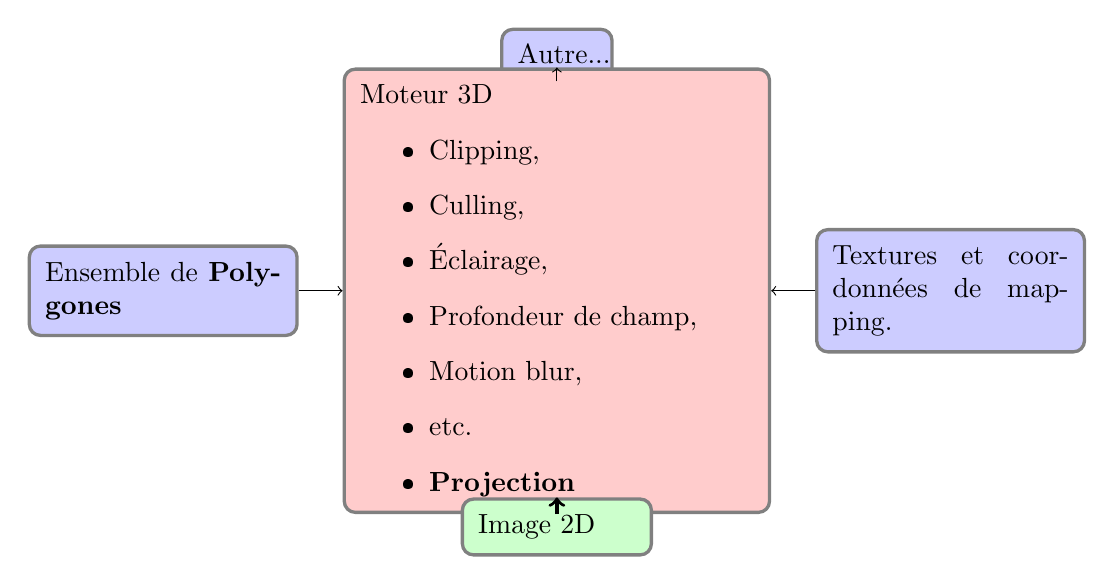
\begin{tikzpicture}
  [entree/.style={
    draw=black!50,
    fill=blue!20,
    rectangle,
    rounded corners,
    inner sep=.2cm,
    very thick}, systeme/.style={
    draw=black!50,
    fill=red!20,
    rectangle,
    rounded corners,
    inner sep=.2cm,
    very thick}, sortie/.style={
    draw=black!50,
    fill=green!20,
    rectangle,
    rounded corners,
    inner sep=.2cm,
    very thick}]

  \node [entree] at (-5,0) (polygone) {
  \begin{minipage}{3cm}
    Ensemble de \textbf{Polygones}
  \end{minipage}
  };

  \node [entree] at (5,0) (textures) {
  \begin{minipage}{3cm}
    Textures et coordonnées de mapping.
  \end{minipage}
  };

  \node [entree] at (0,3) (other) {
  \begin{minipage}{1cm}
    Autre...
  \end{minipage}
  };

  \node [systeme] (engine) {
  \begin{minipage}{5cm}
    Moteur 3D 
    \begin{itemize}
      \item Clipping,
      \item Culling,
      \item Éclairage,
      \item Profondeur de champ,
      \item Motion blur,
      \item etc.
      \item \textbf{Projection}
    \end{itemize}
  \end{minipage}
  };

  \node [sortie] at (0,-3) (image) {
  \begin{minipage}{2cm}
    Image 2D
  \end{minipage}
  };

  \draw [->] (polygone) -- (engine);
  \draw [->] (textures) -- (engine);
  \draw [->] (other) -- (engine);
  \draw [very thick, ->] (engine) -- (image);
\end{tikzpicture}
\caption{Représentation grossière du pipeline de rendu via la
rasterisation\label{rasterisationPipeline}}
\end{center}
\end{figure}


L'avantage de cette technique vient du fait que les calculs sont très
aisément parallélisables. Nous assistons d'ailleurs à un développement de
technologie dans ce sens : Les \gls{GPU} sont devenu de vraies collections de
processeurs.

\newpar Mais cette technique n'offre pas que des avantages. En effet, la
compleification des scènes en 3D et surtout la demande du publique pour des
rendu encore plus réaliste pousse dans ses retranchement le matériel et les
logiciels de visualisation 3D. Mais depuis quelques plus de 30 ans
\cite{Whitted1980}, chercheurs et ingénieurs développent une technique de
rendu simple mais très puissante : Le \raytracing !

\subsection{Le \raytracing ?}

\subsection{Objectifs du projet}
Les objectifs du projet sont nombreux, aussi bien sur le plan de
l'architecture logiciel, que de la gestion de projet ou encore u
développement.

\paragraph{Architecture logiciel}
Un des buts principal du projet (si ce n'est le but principal du projet) est
de créer un programme ouvert à l'extension et pouvant servir de base à la
création d'un \raytracing plus évolué, ou plus rapide, ou plus facile à
utiliser, etc.

\paragraph{Portabilité}
Afin d'être le plus portable possible, j'ai décidé d'utiliser un mélange
d'outils standards comme :
\begin{itemize}
  \item C/C++ : Compilable sur presque toutes les plateformes.
  \item Les autotools\footnote{\url{http://sources.redhat.com/autobook/}} :
  Système de build standard et ne nécessitant aucun autre programme que make
  et bash.
  \item Boost : La bibliothèque C++ de référence.
  \item libpng/libjpg : Pour l'import texture et l'export des résultats.
  \item lib3ds : Pour l'importation des modèles 3D.
\end{itemize}

\paragraph{Gestion de projet}
J'ai réalisé ce projet seul du 24 Septembre au 1 Décembre en utilisant un
style de développement \gls{XP}\footnote{\url{http://www.extremeprogramming.org/}}.
Le gestionnaire de version utilisé est git et le projet ainsi que son
\href{http://digitalguru.github.com/LyonRayTracer}{site web} sont hébergés sur
GitHub.

\paragraph{Implémentation}
Il était pour moi primordial de respecter tout au long de ce projet des
\eng{guidelines} afin d'assurer une cohérence de tout le code (de plusieurs
miliers de lignes tout de même). La documentation fait aussi partie intégrante
du processus de développement et la génération de celle-ci fait partie du
\eng{pipeline} de compilation.

\paragraph{Fonctionnalité du ray tracer}
Reprenons les objectifs fixés dans le sujet :
\begin{enumerate}
  \item Un moteur de \raytracing ``classique''.\textcolor[rgb]{0.0, 0.9, 0.2}{\checkmark}
  \item La gestion de primitives (sphères, plan, tores, et en général toutes
    les figures ayant une représentation paramétrique).\textcolor[rgb]{0.0, 0.9, 0.2}{\checkmark}
  \item La gestion de plusieurs types de caméras : Orthographique,
    perspective, \etc\textcolor[rgb]{0.0, 0.9, 0.2}{\checkmark}
  \item La gestion de plusieurs types de lumières : Point, plan, sphérique,
    \etc.\textcolor[rgb]{0.0, 0.9, 0.2}{\checkmark}
  \item La gestion d'au moins un format de représentation polygonale.\textcolor[rgb]{0.0, 0.9, 0.2}{\checkmark}
  \item La mise en place des structures accélératrices.\textcolor[rgb]{0.0, 0.9, 0.2}{\checkmark}
\end{enumerate}

\newpar J'ai aussi pris le temps d'implémenter :
\begin{enumerate}
  \item Un chargeur de scènes XML.
  \item La lecture et l'écriture d'images au format PNG ou JPG (avec la
  possibilité d'ajouter d'autre formats).
  \item La gestion des textures.
  \item Le \gls{supersampling}.
\end{enumerate}

\subsection{Non-objectifs}
Comme dans tout projet, celui-ci possède des non-objectifs, \ie des objectifs
que j'ai décider volontairement de ne pas atteindre, ou en tout cas de ne pas
viser. 

\newpar D'abord, la vitesse d'exécution. Les \eng{raytracers} commerciaux sont
de réelles prouesses d'ingénierie et d'optimisation et j'ai considérer que
l'optimisation de tels programme sort du contexte d'un projet personnel.
